\begin{figure*}[!t]
\centering
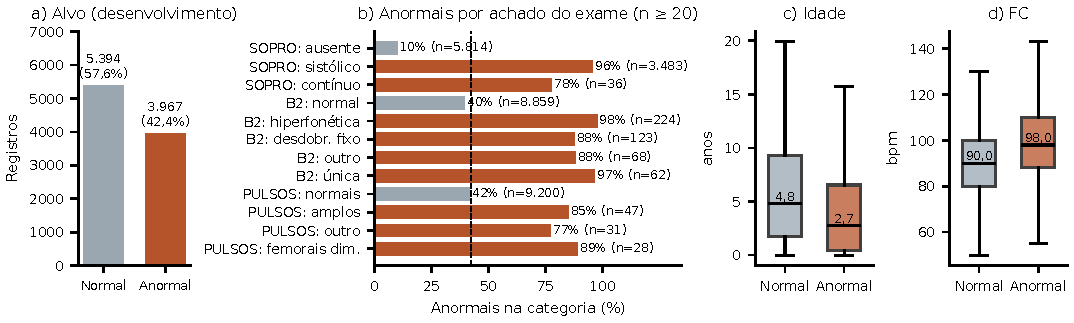
\includegraphics[width=\textwidth]{eda_alvo_achados.pdf}
\caption{Conjunto de desenvolvimento. (a) Distribuição do alvo. (b) Percentual de anormais em cada categoria de SOPRO, B2 e PULSOS com pelo menos 20 registros; a linha tracejada marca a proporção geral (\pctAnormal\%). (c, d) Idade e frequência cardíaca por classe; as caixas vão do primeiro ao terceiro quartil, o traço é a mediana e os pontos atípicos não são desenhados.}
\label{fig:eda}
\end{figure*}

\subsection{Origem e composição}
A fonte tem \recNSource{} registros e 21 atributos \cite{tema,dict}: identificação (ID, Atendimento, DN), antropometria (Peso, Altura, IMC), IDADE, SEXO, sinais vitais (pressões sistólica e diastólica, PAS e PAD, e frequência cardíaca, FC), a classificação de pressão arterial PPA \cite{ppa}, achados do exame físico (SOPRO, segunda bulha B2 e PULSOS), sintomas da história da doença atual (HDA1 e HDA2), Convênio, os motivos de encaminhamento (MOTIVO1 e MOTIVO2) e o alvo. Há \recNUnlabelled{} registros sem rótulo, que ficam fora da classificação supervisionada. Dos \recNLabelledAdois{} rotulados, \nDev{} formam o conjunto de desenvolvimento e \nTest{} formam o teste histórico, separado em uma fase anterior do projeto; \nRetirado{} registro idêntico a outro do teste foi retirado do desenvolvimento. O desenvolvimento tem \nNormal{} registros \textit{Normal} e \nAnormal{} \textit{Anormal} (\pctAnormal\%), um desequilíbrio moderado (Fig.~\ref{fig:eda}a).

\subsection{Descobertas da análise exploratória}
Os achados do exame físico separam as classes com nitidez (Fig.~\ref{fig:eda}b). Entre os \sopSisN{} registros com sopro sistólico, \sopSisPct\% são anormais; entre os \sopAusN{} sem sopro, \sopAusPct\%. B2 normal tem \btwoNormPct\% de anormais e B2 hiperfonética, \btwoHiperPct\%. Pulsos alterados também se concentram na classe anormal, mas são raros.

As crianças com rótulo anormal são mais novas (Fig.~\ref{fig:eda}c): a mediana de idade é \idadeMedAnormal{} anos contra \idadeMedNormal{}, e \menosUmAnoAnormal\% dos anormais têm menos de um ano, contra \menosUmAnoNormal\% dos normais. A FC mediana é \fcMedAnormal{} bpm nos anormais e \fcMedNormal{} bpm nos normais, com intervalos interquartis sobrepostos (\fcQumAnormal--\fcQtresAnormal{} e \fcQumNormal--\fcQtresNormal{} bpm). Como a FC de repouso cai com a idade, parte dessa diferença acompanha a idade.

A falta de dados é desigual: PAS falta em \missPAS\% dos registros, PPA em \missPPA\%, HDA1 em \missHDAum\% e HDA2 em \missHDAdois\%, enquanto SOPRO, B2 e PULSOS faltam em menos de 1\%.

\subsection{Vazamento de informação}
Consideramos vazamento todo atributo indisponível no momento da previsão ou que já contenha a conclusão diagnóstica. A Tabela~\ref{tab:policy} resume a decisão para os 21 atributos. MOTIVO1 e MOTIVO2 trazem textos como ``cardiopatia já estabelecida'' e ``cardiopatia congênita''; a A1 já havia apontado esse risco, e cada um sozinho atinge acurácia balanceada (BA) de \probeMotivoUm\% e \probeMotivoDois\% em um teste exploratório com uma árvore rasa. Convênio descreve a origem do paciente e o caminho de encaminhamento, não a criança: os \susN{} registros do SUS no desenvolvimento têm \susPct\% de anormais, o que reflete quem encaminha, e não o que se observa no atendimento. HDA2 tem \missHDAdois\% de ausentes e sai pela regra da A1 de excluir atributos com mais de 50\% de ausência.

Os achados de exame (SOPRO, B2, PULSOS), os sintomas relatados (HDA1) e a PPA, calculada a partir de PAS, PAD, idade, sexo e altura \cite{ppa}, são coletados durante o atendimento, antes do laudo. São exatamente a informação que o cardiologista usa para decidir a investigação \cite{guideline}. SOPRO sozinho atinge BA de \probeSopro\% no mesmo teste exploratório; isso mede poder preditivo de um dado disponível, não vazamento. O cenário principal, \clinico{}, mantém esses atributos. Os cenários \fisio{} e \strict{} servem de análise de sensibilidade: retiram os achados de exame e, no segundo caso, também os sinais vitais.

\begin{table}[!t]
\centering
\caption{Decisão sobre os 21 atributos originais}
\label{tab:policy}
\footnotesize
\begin{tabular}{@{}p{0.36\columnwidth}p{0.59\columnwidth}@{}}
\toprule
Atributos & Decisão \\
\midrule
\textit{NORMAL X ANORMAL} & Alvo. \\
ID & Fora: identificador. \\
Atendimento, DN & Fora como datas; usadas para conferir IDADE. \\
Convênio & Fora: origem do paciente, não achado clínico. \\
MOTIVO1, MOTIVO2 & Fora: conteúdo diagnóstico explícito. \\
HDA2 & Fora: mais de 50\% de ausentes. \\
SOPRO, B2, PULSOS, HDA1, PPA & Em \clinico{}: coletados antes do laudo. \\
IMC, PAS, PAD, FC & Em \clinico{} e \fisio{}. \\
Peso, Altura, IDADE, SEXO & Nos três cenários. \\
\bottomrule
\end{tabular}
\end{table}
